% paper.tex — "A Certificate-First x86-64 Superoptimizer with a Calibrated
% Comparison Against GCC"
%
% BUILD: ./build.sh   (re-checks every artifact, re-runs the claims audit,
% re-extracts every number into generated/, then compiles).
%
% TRACEABILITY CONTRACT: no number in this document is hand-typed. All
% quantitative claims arrive via generated/numbers.tex (single macros),
% generated/*-table.tex (table bodies), generated/*.asm (instruction
% sequences), and generated/*-chart.tex (plot coordinates), all emitted
% by extract_data.py from the committed JSONL artifacts and markdown
% record. If a value cannot be traced, extract_data.py aborts the build
% rather than letting an untraceable number through.
%
% HOUSE STYLE: em-dash free; the stock constructions listed in
% check_style.py are banned. The build's style gate enforces both on
% the rendered PDF.

\documentclass[journal,10pt]{IEEEtran}

% ------------------------------------------------------------- typography
\usepackage{libertinus}          % Libertinus Serif body + math,
                                 % Libertinus Sans for headings
\usepackage{cite}
\usepackage{amsmath,amssymb}
\usepackage{graphicx}
\usepackage{textcomp}
\usepackage{xcolor}
\usepackage{colortbl}
\usepackage{array}
\usepackage{booktabs}
\usepackage{listings}
\usepackage{tikz}
\usetikzlibrary{arrows.meta,positioning,shapes.geometric,calc}
\usepackage{pgfplots}
\pgfplotsset{compat=1.16}
\usepackage{titlesec}
\usepackage{microtype}
\usepackage{csquotes}
\usepackage{tcolorbox}
\tcbuselibrary{skins,breakable}
\usepackage{fontawesome5}
\usepackage{enumitem}
\usepackage[hidelinks]{hyperref}

% --------------------------------------------------------------- palette
% One five-colour system for every figure, diagram, and table rule.
\definecolor{ink}{HTML}{1B2A38}      % headings, rules, primary structure
\definecolor{accent}{HTML}{0F6B52}   % verified / beaten
\definecolor{steel}{HTML}{1F5C99}    % matched / secondary structure
\definecolor{neutral}{HTML}{6E7479}  % honest no-improvement / metadata
\definecolor{ochre}{HTML}{B4652A}    % benchmark / measurement accent
% figure-facing aliases (single source of truth above)
\definecolor{beatencolor}{HTML}{0F6B52}
\definecolor{matchedcolor}{HTML}{1F5C99}
\definecolor{honestcolor}{HTML}{6E7479}
\definecolor{pymcolor}{HTML}{1B2A38}
\definecolor{opcodecolor}{HTML}{1F5C99}
\definecolor{tlWone}{HTML}{6E7479}
\definecolor{tlsearch}{HTML}{1F5C99}
\definecolor{tlverify}{HTML}{0F6B52}
\definecolor{tlbench}{HTML}{B4652A}
\colorlet{pymA}{pymcolor!85}
\colorlet{pymB}{pymcolor!70}
\colorlet{pymC}{pymcolor!60}
\colorlet{pymD}{pymcolor!50}
\colorlet{pymE}{pymcolor!40}
\colorlet{pymF}{pymcolor!30}

% table rules in the structural ink colour
\arrayrulecolor{ink}

% --------------------------------------------------------- heading style
\titleformat{\section}[block]
  {\sffamily\bfseries\color{ink}\large}{\thesection}{0.7em}{}
  [\vspace{1pt}{\color{ink}\titlerule[0.7pt]}]
\titlespacing*{\section}{0pt}{2.4ex plus 0.6ex minus 0.3ex}{1.2ex}
\titleformat{\subsection}[block]
  {\sffamily\bfseries\color{ink}\normalsize}{\thesubsection}{0.6em}{}
\titlespacing*{\subsection}{0pt}{1.8ex plus 0.4ex minus 0.2ex}{0.8ex}
\titleformat{\subsubsection}[runin]
  {\sffamily\bfseries\color{steel}\small}{}{0pt}{}[.]
\titlespacing*{\subsubsection}{0pt}{1.4ex plus 0.3ex minus 0.2ex}{0.5em}

% --------------------------------------------------- running footers
\makeatletter
\def\@oddfoot{\footnotesize\color{neutral}%
  \hfil Certificate-First x86-64 Superoptimizer \quad\textbar\quad \thepage \hfil}
\def\@evenfoot{\footnotesize\color{neutral}%
  \hfil \thepage \quad\textbar\quad Certificate-First x86-64 Superoptimizer \hfil}
% title page style: class default headers, our footer added
\def\ps@IEEEtitlepagestyle{%
  \def\@oddhead{\hbox{}\@IEEEheaderstyle\leftmark\hfil\thepage}\relax
  \def\@evenhead{\@IEEEheaderstyle\thepage\hfil\leftmark\hbox{}}\relax
  \def\@oddfoot{\footnotesize\color{neutral}%
    \hfil Certificate-First x86-64 Superoptimizer \quad\textbar\quad \thepage \hfil}%
  \def\@evenfoot{\footnotesize\color{neutral}%
    \hfil \thepage \quad\textbar\quad Certificate-First x86-64 Superoptimizer \hfil}}
\makeatother

% ------------------------------------------------------------- listings
% IEEEtran hardcodes "Abstract---" and "Index Terms---"; house style
% admits no em dashes, so the two environments are redefined with a colon.
\makeatletter
\def\abstract{\normalfont
    \@IEEEabskeysecsize\bfseries\textit{\abstractname:}\hspace{0.33em}\relax
    \@IEEEgobbleleadPARNLSP}
\def\endabstract{\relax\ifCLASSOPTIONconference\vspace{0ex}\else\vspace{1.34ex}\fi
    \par\normalfont\normalsize}
\def\IEEEkeywords{\normalfont
    \@IEEEabskeysecsize\bfseries\textit{\IEEEkeywordsname:}\hspace{0.33em}\relax
    \@IEEEgobbleleadPARNLSP}
\def\endIEEEkeywords{\relax\ifCLASSOPTIONtechnote\vspace{1.34ex}\else\vspace{0.67ex}\fi
    \par\normalfont\normalsize}
\makeatother

\lstdefinestyle{asmstyle}{
  basicstyle=\ttfamily\fontsize{7.5}{9}\selectfont,
  keywordstyle=\color{opcodecolor}\bfseries,
  keywords={movq,movabsq,addq,subq,andq,orq,xorq,cmpq,shrq,shlq,salq,sarq,
            leaq,negq,notq,seta,setb,sete,setl,setae,setg,setle,setnb,
            setne,setbe,setge,setnle,setnl,setng,setna,setnae,setc,setnc,
            cmovbq,cmovleq,cmovnbq,cmovgq,cmovneq,cmovaeq,cmovbeq,cmovlq,
            imulq,divq,idivq},
  sensitive=false,
  showstringspaces=false,
  columns=fixed,
  basewidth=0.5em,
  xleftmargin=2pt,
  framexleftmargin=2pt,
  keepspaces=true
}

% ------------------------------------------------------------- extracted data
% generated by extract_data.py — the paper's only numeric source
% every macro traces to a committed artifact or document
\newcommand{\IdenticalLevels}{true}
\newcommand{\CompilerVersion}{gcc (Ubuntu 15.2.0-16ubuntu1) 15.2.0}
\newcommand{\NumFunctions}{23}
\newcommand{\NumBaselines}{46}
\newcommand{\NumTestcases}{43\,494}
\newcommand{\NumWitnesses}{20\,538}
\newcommand{\NumBeaten}{3}
\newcommand{\NumMatched}{13}
\newcommand{\NumHonest}{7}
\newcommand{\TotalCandidates}{14\,216\,086}
\newcommand{\TotalOptima}{26}
\newcommand{\MinCandidates}{472}
\newcommand{\MinCandFn}{sign\_mask}
\newcommand{\MaxCandidates}{5\,104\,879}
\newcommand{\MaxCandFn}{sat\_add}
\newcommand{\MedianOptChainSec}{120}
\newcommand{\MedianSynthChainSec}{60}
\newcommand{\GccLenIabs}{5}
\newcommand{\OursLenIabs}{3}
\newcommand{\SpecPerfIabs}{5}
\newcommand{\PerfIabs}{3}
\newcommand{\GccLenPthirteen}{5}
\newcommand{\OursLenPthirteen}{4}
\newcommand{\SpecPerfPthirteen}{5}
\newcommand{\PerfPthirteen}{4}
\newcommand{\GccLenPnineteen}{9}
\newcommand{\OursLenPnineteen}{8}
\newcommand{\SpecPerfPnineteen}{9}
\newcommand{\PerfPnineteen}{8}
\newcommand{\StragglerChains}{8}
\newcommand{\StragglerSeconds}{300}
\newcommand{\NumSynth}{4}
\newcommand{\BulkPrograms}{2\,000\,000}
\newcommand{\BulkEvals}{4\,000\,000}
\newcommand{\ZSolverQueries}{8000}
\newcommand{\GridPrograms}{5344}
\newcommand{\SelfPrograms}{2000}
\newcommand{\PairVerdicts}{18}
\newcommand{\HwCases}{64\,000}
\newcommand{\HwFlagComps}{242\,156}
\newcommand{\HwMemCases}{8000}
\newcommand{\HwMemDef}{2143}
\newcommand{\OracleFns}{46}
\newcommand{\OracleCases}{92\,000}
\newcommand{\Exclusions}{16}
\newcommand{\EnumCandidates}{218\,955}
\newcommand{\EnumChainA}{278\,377}
\newcommand{\EnumChainB}{279\,088}
\newcommand{\EnumChainC}{249\,223}
\newcommand{\EnumChainD}{218\,955}
\newcommand{\RecheckTotal}{114\,295}
\newcommand{\RecheckFailed}{0}
\newcommand{\AuditChecks}{485}
\newcommand{\NumTests}{66}
\newcommand{\NumLedgerRows}{34}

% generated by extract_data.py
% NOTE: pgfplots assigns yticklabels bottom-up (tick 1 first), while the
% data places the first row at the top (y = N). The label list is
% therefore emitted REVERSED so tick 23 reads the first row.
\def\RatioNames{select\_bits,p23\_popcnt\_bytes,p17\_turn\_off\_run,p15\_avg\_ceil,p07\_isolate\_rightmost0,next\_pow2,avg,umin,umax,turn\_off\_rightmost,smin,sign\_mask,sat\_add,p16\_umax\_bitwise,p08\_mask\_trailing\_zeros,p06\_turn\_on\_rightmost0,p05\_smear\_rightmost,p04\_mask\_lowest\_ones,p02\_test\_2n\_minus\_1,lowest\_set\_bit,p19\_exchange\_fields,p13\_sign,iabs}
      % \RatioNames for Fig. ratio
% generated by extract_data.py: enumeration_summary.candidates_total (O2)
% labels reversed for the same bottom-up pgfplots assignment as Fig. ratio
\def\CandNames{sat\_add,lowest\_set\_bit,p08\_mask\_trailing\_zeros,smin,umin,p16\_umax\_bitwise,umax,p04\_mask\_lowest\_ones,p06\_turn\_on\_rightmost0,p05\_smear\_rightmost,turn\_off\_rightmost,p02\_test\_2n\_minus\_1,sign\_mask}
 % \CandNames for Fig. candidates
% generated by extract_data.py — invoke \ResultsTableBody inside the tabular
\newcommand{\ResultsTableBody}{%
iabs & P9 & 5 & \textcolor{beatencolor}{beaten} & 3 & perf 5 \ensuremath{\rightarrow} 3 via MCMC (z3-equivalent) \\
p13\_sign & P13 & 5 & \textcolor{beatencolor}{beaten} & 4 & perf 5 \ensuremath{\rightarrow} 4 via MCMC (z3-equivalent) \\
p19\_exchange\_fields & P19 & 9 & \textcolor{beatencolor}{beaten} & 8 & perf 9 \ensuremath{\rightarrow} 8 via MCMC (z3-equivalent) \\
lowest\_set\_bit & P3 & 3 & \textcolor{matchedcolor}{matched} & 3 & 871,298 cand., 6 z3 \\
p02\_test\_2n\_minus\_1 & P2 & 2 & \textcolor{matchedcolor}{matched} & 2 & 1,715 cand., 1 z3 \\
p04\_mask\_lowest\_ones & P4 & 2 & \textcolor{matchedcolor}{matched} & 2 & 2,695 cand., 1 z3 \\
p05\_smear\_rightmost & P5 & 2 & \textcolor{matchedcolor}{matched} & 2 & 2,205 cand., 1 z3 \\
p06\_turn\_on\_rightmost0 & P6 & 2 & \textcolor{matchedcolor}{matched} & 2 & 2,205 cand., 1 z3 \\
p08\_mask\_trailing\_zeros & P8 & 3 & \textcolor{matchedcolor}{matched} & 3 & 555,680 cand., 1 z3 \\
p16\_umax\_bitwise & P16 & 3 & \textcolor{matchedcolor}{matched} & 3 & 139,768 cand., 1 z3 \\
sat\_add & n/a & 3 & \textcolor{matchedcolor}{matched} & 3 & 5,104,879 cand., 2 z3 \\
sign\_mask & n/a & 2 & \textcolor{matchedcolor}{matched} & 2 & 472 cand., 1 z3 \\
smin & n/a & 3 & \textcolor{matchedcolor}{matched} & 3 & 146,108 cand., 3 z3 \\
turn\_off\_rightmost & P1 & 2 & \textcolor{matchedcolor}{matched} & 2 & 1,715 cand., 1 z3 \\
umax & n/a & 3 & \textcolor{matchedcolor}{matched} & 3 & 139,507 cand., 1 z3 \\
umin & n/a & 3 & \textcolor{matchedcolor}{matched} & 3 & 139,796 cand., 1 z3 \\
avg & P14 & 5 & \textcolor{honestcolor}{no improve} & 5 & MCMC budget, no verified improvement \\
next\_pow2 & P24 & 20 & \textcolor{honestcolor}{no improve} & 20 & MCMC budget, no verified improvement \\
p07\_isolate\_rightmost0 & P7 & 4 & \textcolor{honestcolor}{no improve} & 4 & MCMC budget, no verified improvement \\
p15\_avg\_ceil & P15 & 5 & \textcolor{honestcolor}{no improve} & 5 & MCMC budget, no verified improvement \\
p17\_turn\_off\_run & P17 & 4 & \textcolor{honestcolor}{no improve} & 4 & MCMC budget, no verified improvement \\
p23\_popcnt\_bytes & P23 & 16 & \textcolor{honestcolor}{no improve} & 16 & MCMC budget, no verified improvement \\
select\_bits & n/a & 4 & \textcolor{honestcolor}{no improve} & 4 & MCMC budget, no verified improvement \\
}
    % defines \ResultsTableBody
% generated by extract_data.py — invoke \StragglerTableBody inside the tabular
\newcommand{\StragglerTableBody}{%
avg (-O2) & 5 & 5 & no\_improvement \\
avg (-O3) & 5 & 5 & no\_improvement \\
next\_pow2 (-O2) & 20 & 20 & no\_improvement \\
next\_pow2 (-O3) & 20 & 20 & no\_improvement \\
select\_bits (-O2) & 4 & 4 & no\_improvement \\
select\_bits (-O3) & 4 & 4 & no\_improvement \\
}
  % defines \StragglerTableBody
% generated by extract_data.py — invoke \LedgerTableBody inside the tabular
\newcommand{\LedgerTableBody}{%
1 & Concrete IMUL zero-extended operands into i128 ;  wrong CF/OF for negative operands & corner unit test & random states hit negative\ensuremath{\times}negative rarely in the flag bits that differ; symbolic construction was \emph{right}, so differential testing would eventually catch it but the corner test did first \\
3 & \texttt{msb()}/\texttt{bit()} compared a 1-bit extract against a 64-bit constant ;  z3 sort error & miter self-checks (grid) & all \emph{folding} was correct; only the printed SMT was wrong, so layers 2/6 saw nothing \\
8 & Enumerator optimized the program \emph{as written} and exposed a desc/spec mismatch (\texttt{shl \$63} extracts bit 0, not 63) & the enumerator itself (enumeration layer) & the spec was wrong; no test layer can catch an author's intent error ;  the certificate is about the program text, which is why the tool was right to optimize the text \\
11 & Unsigned \#DE bound printed as the 128-bit all-ones literal instead of zero-extended u64::MAX ;  every quotient \ensuremath{\leq} 2\textsuperscript{128} counted as defined & z3-sampled differential (1,733 discrepancies) & the \emph{fold} was correct; concrete/fold differential (layer 2) saw perfect agreement \\
13 & Load64 printer byte-rotated the concat chain (s6..s0,s7) & z3-sampled differential (384 cases) & folds were right AND the miter stayed sound (both sides rotate identically) ;  only cross-checking z3's evaluated memory against concrete bytes exposed it \\
15 & Signed \#DE lower bound used \texttt{bvsgt} ;  the exact INT64\_MIN quotient boundary was misclassified & z3-sampled differential (1 case in 8,000) & a one-in-2\textsuperscript{64}-ish boundary; random sampling hit it once \\
17 & Signed \#DE \textbf{upper} bound used \texttt{bvslt} ;  quotient exactly i64::MAX (defined) rejected as undefined; the miter "counterexampled" a pair whose outputs were equal. & \textbf{hand-picked broken pair, first run} (division/memory review-gap closure) & survived 8,000 random z3 samples \emph{and} the earlier boundary fix's symmetric twin: random inputs essentially never make the quotient exactly i64::MAX. \\
22 & An early prose report mis-transcribed a counterexample input & \textbf{external hand-verification} & the machine outputs were right; the \emph{report} was the bug ;  this created the artifact-of-record pipeline (ADR-009) \\
23 & The i64::MAX boundary bug's discovery witness (row 17) was \textbf{destroyed}: the failing run's artifact was overwritten by the truncating re-run and then \texttt{rm}'d before the commit. & external audit of the \emph{audit machinery} & nothing in the pyramid watches the debugging workflow itself; failure evidence produced outside the artifact pipeline has no protection. \\
24 & Model: entry flags treated as defined-false ;  candidates could read RFLAGS at function entry and get fake constants (\texttt{sete \%rax} at entry \ensuremath{\rightarrow} constant 0). & \textbf{compiler-output integration} (compiler-baseline phase) & every earlier layer used hand-written specs that masked the issue ;  exactly why "beat the compiler" was a required phase, not a nice-to-have \\
32 & The first full-provenance run claimed \textbf{p23\_popcnt\_bytes 16 \ensuremath{\rightarrow} 14} ;  but three of the 14 forms were \texttt{andq \$imm64} (\texttt{\$0x5555555555555555}, \texttt{\$0xcccccccccccccccd}, \texttt{\$0x3333333333333333}), which real x86 cannot encode: AND takes sign-extended imm32 only, which is exactly why gcc materialized those constants with movabsq. & inspection of the claimed program against x86 encoding rules & the fifth instance of model-vs-world: a verifier-perfect equivalence proof over a universe that quietly contains forms the hardware doesn't have. \\
33 & The second full-provenance run claimed \textbf{p13\_sign 5 \ensuremath{\rightarrow} 4} ;  a genuine four-instruction sign function (\texttt{negq; setl; movq \$-1, \%rsp; cmovgq}) except that it materialized its \ensuremath{-}1 \textbf{in \%rsp}: in-model perfectly correct (v0 treats all 16 GPRs as equal and the live-out was RAX only, and z3 proved the equivalence) but a real function body that sets RSP=\ensuremath{-}1 jumps through the return address on \texttt{ret} ;  it is not a drop-in replacement for gcc's function at all. & inspection of the new claimed program against the ABI (the same discipline as row 32) & the sixth instance, and the second in one run: the model's register file is an abstraction, and "equivalent, live-out RAX" quietly diverges from "equivalent function" whenever the winner touches RSP/RBP/RBX/R12-R15. \\
34 & \texttt{audit\_claims.py} printed its \textbf{AUDIT PASSED verdict mid-file} ;  right after the optimize section ;  and \texttt{sys.exit(0)}-by-default meant every check added after that point (all of the compiler-batch sections) could print \texttt{FAIL} lines without changing the exit code. & extending the audit for the full batch (its own probe output) & the same failure family as row 28, one layer up: the \emph{verifier of the numbers} had a number of its own that didn't decompose to what it checked. \\
}
     % defines \LedgerTableBody

\hyphenpenalty=1000
\setlist[itemize]{leftmargin=1.15em,itemsep=1.6pt,topsep=2.5pt,parsep=0pt}
\setlist[enumerate]{leftmargin=1.5em,itemsep=1.6pt,topsep=2.5pt,parsep=0pt}
\setlength{\abovedisplayskip}{4.5pt plus 1pt minus 1pt}
\setlength{\belowdisplayskip}{4.5pt plus 1pt minus 1pt}

\begin{document}

\title{A Certificate-First x86-64 Superoptimizer with a Calibrated
Comparison Against GCC}

\author{Imtamum~Hosen~Inan%
\thanks{Manuscript prepared November 2026. Copyright \copyright\ 2026
Imtamum Hosen Inan. The complete project record (11 architecture
decision records, a \NumLedgerRows{}-row verification ledger, and nine
machine-checkable JSONL artifacts of record) is committed alongside the
source in the Isuperoptimizer repository. Every number printed in this
paper was machine-extracted from those artifacts by
\texttt{extract\_data.py}; the build refuses to complete if any claimed
value cannot be traced.}%
\thanks{Independent research project.}}

\markboth{Certificate-First x86-64 Superoptimizer, November 2026}%
{Inan: Certificate-First x86-64 Superoptimizer}

\maketitle

\begin{abstract}
Superoptimization searches for the shortest instruction sequence that
implements a function, and its results are usually reported in prose.
This paper documents Isuperoptimizer, a seven-week project that treats
reporting as part of the experimental apparatus. The system implements
a total-semantics model of a curated x86-64 subset, an SMT equivalence
miter built on z3, an exhaustive enumerator that emits optimality
certificates, and an MCMC search faithful to STOKE's published
hyperparameters. Every result is written to an append-only JSONL
artifact of record that independent tools re-verify from the log alone.
Measured against real \CompilerVersion{} output over the 25-program
Hacker's Delight benchmark provenance of Gulwani et al.\ at both
\mbox{-O2} and \mbox{-O3}, \NumBeaten{} of \NumFunctions{} surviving
functions are beaten with z3-verified, x86-encodable, ABI-clean drop-in
replacements, including a \OursLenPthirteen-instruction sign function
and an \OursLenPnineteen-instruction field-exchange. A further
\NumMatched{} functions are matched with exhaustive in-universe
optimality proofs totaling \TotalCandidates{} rejected candidates, and
\NumHonest{} survive honestly, three of them after a seeded-synthesis
second attempt at five times the primary per-chain synthesis budget.
The verification pyramid behind these numbers runs from \NumTests{}
unit tests through \BulkPrograms{}-program differentials and
\HwCases{}-case silicon oracles to \RecheckTotal{} artifact events
re-verified with zero failures, and it caught \NumLedgerRows{} defects,
five of them latent model bugs that flawless testing had hidden. The
methodological result is that when every claim must survive artifact
inspection, the artifacts become trustworthy by construction.
\end{abstract}

\begin{IEEEkeywords}
superoptimization, program verification, SMT solving, x86-64,
compiler optimization, reproducible research
\end{IEEEkeywords}

\begin{tcolorbox}[enhanced, colback=white, colframe=ink!20,
                  boxrule=0.5pt, arc=3pt, left=4pt, right=4pt,
                  top=6pt, bottom=6pt]
\begin{minipage}[t]{0.48\columnwidth}\centering
{\sffamily\bfseries\fontsize{17}{19}\selectfont\color{accent}%
\NumBeaten/\NumFunctions}\\[1pt]
{\sffamily\scriptsize\color{neutral}functions beaten\\with verified drop-ins}
\end{minipage}\hfill
\begin{minipage}[t]{0.48\columnwidth}\centering
{\sffamily\bfseries\fontsize{17}{19}\selectfont\color{steel}%
\NumMatched/\NumFunctions}\\[1pt]
{\sffamily\scriptsize\color{neutral}matched with\\optimality proofs}
\end{minipage}\\[5pt]
\begin{minipage}[t]{0.48\columnwidth}\centering
{\sffamily\bfseries\fontsize{17}{19}\selectfont\color{ink}%
\RecheckTotal}\\[1pt]
{\sffamily\scriptsize\color{neutral}events re-verified\\zero failures}
\end{minipage}\hfill
\begin{minipage}[t]{0.48\columnwidth}\centering
{\sffamily\bfseries\fontsize{17}{19}\selectfont\color{ochre}%
\NumLedgerRows}\\[1pt]
{\sffamily\scriptsize\color{neutral}defects caught by\\the pyramid}
\end{minipage}
\end{tcolorbox}

\vspace{1pt}

\section{Introduction}
\IEEEPARstart{S}{uperoptimization} is the search for the provably
shortest instruction sequence implementing a function. Since
Massalin's superoptimizer \cite{massalin87}, the field has produced
instruction sequences that neither compilers nor textbook authors had
found. Such results are usually reported in prose: a paper asserts
that a sequence is shorter, equivalent, and optimal, and the reader
trusts the authors, the test suite, and the solver.

This project treats that trust as part of the measurement problem.
Weeks of implementation produce search results, but they also produce
transcription errors, verifier-adjacent bugs, self-neutralizing tests,
and model abstractions that license behavior the hardware does not
have. Isuperoptimizer was built around one rule: no claim is ever
retyped from memory. Every headline number is a machine-extracted
property of an append-only JSONL artifact, independent binaries
re-derive every concretely checkable claim from the log alone, and an
external claims audit recomputes the paper's numbers from the committed
files. The build that produced this PDF first re-verified
\RecheckTotal{} artifact events with zero failures and re-ran the
\AuditChecks{}-check audit.

\subsection{Contributions}
\begin{itemize}
\item \textbf{A certificate-first superoptimizer} for a curated
x86-64 subset: total semantics with per-flag definedness, a z3-backed
equivalence miter, an exhaustive backward-liveness enumerator that
rejects every shorter candidate with a logged witness, and an MCMC
search faithful to STOKE's published move set and hyperparameters
\cite{stoke13} (Section~\ref{sec:arch}).
\item \textbf{A seven-layer verification pyramid} in which no layer
trusts another: unit tests, millions-scale concrete-vs-symbolic
differentials, solver-sampled round-trips, a self-verification grid,
hand-picked equivalence and broken pairs, a silicon hardware oracle,
and artifact re-derivation (Section~\ref{sec:pyramid}).
\item \textbf{A calibrated compiler comparison at benchmark scale}:
\NumBeaten{} beaten, \NumMatched{} matched with proof, \NumHonest{}
honestly exhausted, over \NumFunctions{} real compiler-emitted
functions from the Gulwani/STOKE provenance \cite{gulwani11,stoke13}
at both optimization levels (Section~\ref{sec:benchmark}).
\item \textbf{A \NumLedgerRows{}-row defect ledger} with a
failure-shape taxonomy, every row recording what caught the defect and
why the other layers could not (Section~\ref{sec:lessons}). Five
defects were found by reading our own claimed winners against the ISA
and the ABI; the ledger records that the wins reported here survived
three adjudication rounds in which two earlier headline results were
retracted for licensing non-encodable instructions and callee-saved
register writes.
\end{itemize}

\begin{figure*}[!t]
\centering
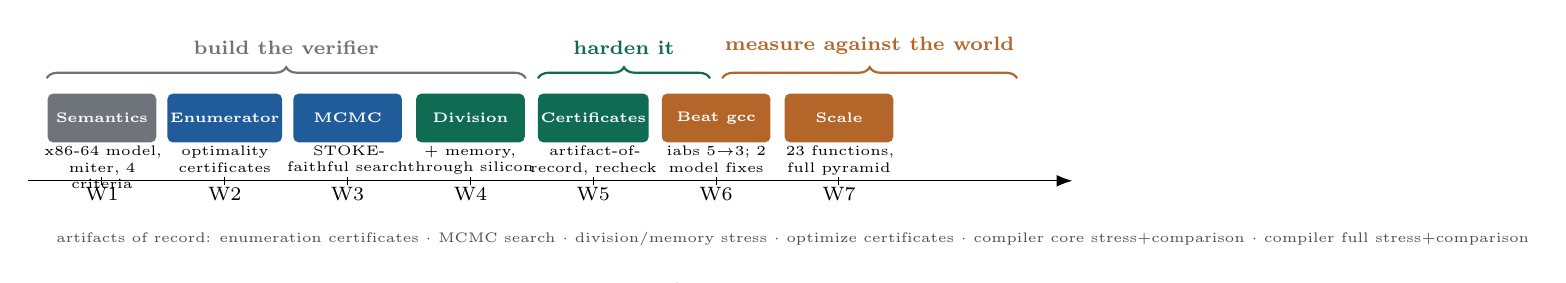
\begin{tikzpicture}[x=0.78cm,y=0.42cm]
  % axis
  \draw[-{Latex[length=2mm]}] (-0.2,0) -- (16.8,0);
  \foreach \w/\lbl in {1/W1,2/W2,3/W3,4/W4,5/W5,6/W6,7/W7}{
    \draw ({2*\w-1},0.12) -- ({2*\w-1},-0.12);
    \node[below,font=\scriptsize,inner sep=1pt] at ({2*\w-1},-0.10) {\lbl};
  }
  % phase bars (phase, color, label above/below)
  \def\bar#1#2#3#4#5{% x-center, color, y, label, artifact
    \node[rectangle, rounded corners=2pt, fill=#2, text=white,
          minimum width=1.38cm, minimum height=0.62cm, font=\tiny\bfseries,
          inner sep=1pt, align=center,
          anchor=center] at (#1,#3) {#4};
    \node[anchor=north, font=\tiny, text width=1.62cm, align=center, text=black]
         at (#1,#3-0.55) {#5};
  }
  \bar{1}{tlWone}{1.9}{Semantics}{x86-64 model, miter, 4 criteria}
  \bar{3}{tlsearch}{1.9}{Enumerator}{optimality certificates}
  \bar{5}{tlsearch}{1.9}{MCMC}{STOKE-faithful search}
  \bar{7}{tlverify}{1.9}{Division}{+ memory, through silicon}
  \bar{9}{tlverify}{1.9}{Certificates}{artifact-of-record, recheck}
  \bar{11}{tlbench}{1.9}{Beat gcc}{iabs 5$\to$3; 2 model fixes}
  \bar{13}{tlbench}{1.9}{Scale}{23 functions, full pyramid}
  % era brackets
  \draw[decorate,decoration={brace,amplitude=4pt},thick,tlWone]
        (0.1,3.1) -- (7.9,3.1)
        node[midway,above=5pt,font=\scriptsize\bfseries,text=tlWone]
        {build the verifier};
  \draw[decorate,decoration={brace,amplitude=4pt},thick,tlverify]
        (8.1,3.1) -- (10.9,3.1)
        node[midway,above=5pt,font=\scriptsize\bfseries,text=tlverify]
        {harden it};
  \draw[decorate,decoration={brace,amplitude=4pt},thick,tlbench]
        (11.1,3.1) -- (15.9,3.1)
        node[midway,above=5pt,font=\scriptsize\bfseries,text=tlbench]
        {measure against the world};
  % artifacts of record
  \node[anchor=west, font=\tiny, text=black!70] at (0.1,-1.75)
    {artifacts of record: enumeration certificates $\cdot$ MCMC search $\cdot$
     division/memory stress $\cdot$ optimize certificates $\cdot$
     compiler core stress+comparison $\cdot$ compiler full stress+comparison};
\end{tikzpicture}
\caption{The seven-week arc. Weeks 1 to 4 built the semantics layer,
miter, enumerator, stochastic search, and the division/memory
extensions; Week 5 turned reporting itself into a verified pipeline
after two incidents (Section~\ref{sec:lessons}); Weeks 6 and 7 pointed
the tool at real compiler output and scaled the comparison to the full
benchmark provenance. One artifact of record was committed in each week
that produced results, and all nine remain re-checkable today. Theme
labels follow the part structure of the project's research log
(Parts I to VII).}
\label{fig:timeline}
\end{figure*}

\section{Background and Related Work}
\label{sec:background}

\subsection{Superoptimization and program synthesis}
Massalin's superoptimizer \cite{massalin87} exhaustively enumerated
instruction sequences over a toy RISC ISA and found provably minimal
programs. Denali \cite{denali02} scaled the approach with goal-directed
enumeration. Peephole superoptimizers \cite{bansal06} enumerate short
instruction sequences to replace compiler-generated patterns, the same
machinery carried to binary translation in \cite{bansal08}, and Souper
\cite{souper} applies solver-based synthesis to compiler IR, where the
rewrite search runs over SSA rather than machine code. The synthesis
literature supplies the broader framing: sketch-based combinatorial
synthesis \cite{sketch06}, syntax-guided synthesis \cite{sygus13},
solver-aided host languages \cite{rosette14}, inductive synthesis
frameworks \cite{flashmeta15}, and general surveys
\cite{gulwani-survey17}. Chlorophyll \cite{chlorophyll14} uses
synthesis to compile for low-power spatial architectures.

Gulwani et al.\ \cite{gulwani11} formulated loop-free synthesis as an
SMT constraint problem and introduced, in its evaluation, a 25-program
benchmark suite drawn from Warren's Hacker's Delight \cite{warren13}.
The programs run from P1 (turn off the rightmost 1-bit) to P25
(compute the high half of a product). STOKE \cite{stoke13} adopted the
same 25 programs; its Figure 11 runs them as p01 to p25 and reports
synthesis timeouts and algorithmically distinct rewrites. This paper
scales the compiler comparison to that full set.

\subsection{Stochastic superoptimization}
STOKE \cite{stoke13} reformulated superoptimization as stochastic
search over a fixed-length program space: MCMC with four proposal
moves (opcode, operand, swap, instruction), an ``improved equality''
metric $\mathrm{eq}'$ that scores register-file Hamming distance
against a testcase set, and a correctness check deferred to an SMT
solver. Its published hyperparameters ($p_{\mathrm{opcode}}=0.16$,
$p_{\mathrm{operand}}=0.5$, $p_{\mathrm{swap}}=0.16$,
$p_{\mathrm{instruction}}=0.16$, $\beta=0.1$, 32 testcases) are the
ones our search implements; every deviation is documented in the
project's ADR-007 and logged in each run's artifact. Schkufza et al.\
extended the approach to floating-point programs with tunable
precision \cite{stokefp14}.

\subsection{Verification of rewrites}
A parallel tradition verifies individual rewrites instead of searching
for them. Translation validation \cite{pnueli98,nec00} checks each
compiler output against its input, equivalence-modulo-inputs testing
\cite{emi14} validates compilers by differentially executing mutated
program variants, and Alive2 \cite{alive2} performs bounded
translation validation for LLVM IR. Verified compilation \cite{leroy09}
and formalized IR semantics \cite{vellvm12} pursue the same goal from
the other direction. Our miter applies the same contract at
instruction granularity, and our claims are certificates over a
declared universe that can be re-derived from committed logs.

\subsection{Differential testing and compiler validation}
Differential testing \cite{mckeeman98} compares independent
implementations on shared inputs. Randomized differential testing
served as a prelude to formal verification \cite{groce07}, and
property-based testing \cite{quickcheck00} established the
generator-and-oracle pattern that our bulk differential implements.
Compiler testing at scale produced Csmith \cite{csmith11}, test-case
reduction \cite{regehr12}, and fuzzer scheduling work \cite{chen13}.
These tools test compilers as wholes. Our pyramid applies the same
differential idea inside a single function's instruction semantics, at
millions of evaluations per run.

\subsection{Reporting discipline}
The project's distinguishing concern, that the report is part of the
experimental apparatus, follows two failures we document rather than
cite: a mis-transcribed counterexample in a prose report (ledger
row~22), and a genuine discovery whose evidence was destroyed by the
debugging workflow around it (row~23). Both incidents created the
artifact-of-record rule under which this paper is built: claims live
in append-only logs, tools re-derive them, and prose cites them.

\section{System Architecture}
\label{sec:arch}

The toolchain is five components, each independently tested, connected
only by the artifact of record.

\subsubsection{Semantics layer} A total-semantics model of a curated
64-bit x86-64 subset: \texttt{movq}, \texttt{movabsq}, ALU and shift
forms, \texttt{leaq}, \texttt{setcc}/\texttt{cmovcc},
\texttt{negq}/\texttt{notq}, two-operand \texttt{imulq}, one-operand
\texttt{divq}/\texttt{idivq}, and load/store over a 256-byte sandbox.
Instruction semantics follow the Intel SDM \cite{intel-sdm} and the
AMD64 programmer's manual \cite{amd-apm}; the SysV ABI \cite{sysvabi}
fixes the calling convention, and the cost model's latency estimates
follow Agner Fog's tables \cite{fog-tables}. The v0 partial-register
ban (ADR-001) rejects every non-64-bit register operand as a hard
parse error, never a silent truncation. Every instruction carries both
concrete and symbolic semantics, including per-flag definedness: the
four RFLAGS bits are modeled as values with definedness predicates, so
reading a flag nobody wrote is a definedness violation rather than a
silent value (Fig.~\ref{fig:miter}). Full-ISA formal semantics exist
\cite{x86sem,x86isa17}, and the x86-TSO model \cite{x86tso10} covers
the memory-ordering side that our straight-line subset does not model.
Our subset is deliberately narrower: total, differentially tested
against silicon, and small enough that every instruction's symbolic
encoding is audited.

\begin{figure}[!t]
\centering
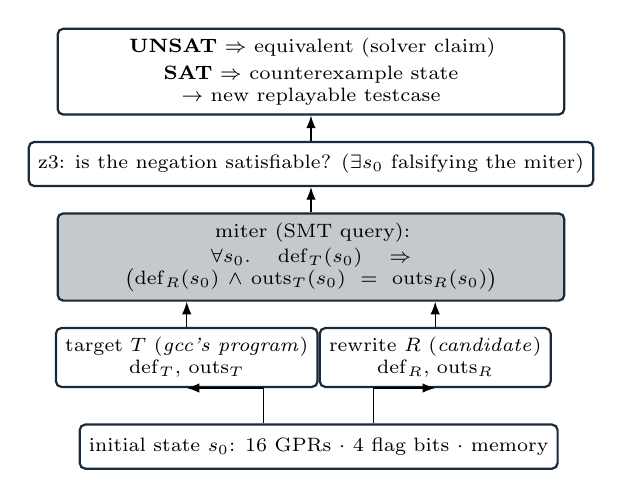
\begin{tikzpicture}[
  node distance=3.2mm,
  box/.style={draw=pymcolor, thick, rounded corners=2pt,
              align=center, font=\scriptsize, minimum height=5.6mm},
  mid/.style={draw=pymcolor, thick, rounded corners=2pt, fill=pymA!30,
              align=center, font=\scriptsize, minimum height=5.6mm,
              text width=62mm},
  res/.style={draw=pymcolor, thick, rounded corners=2pt,
              align=center, font=\scriptsize, minimum height=5.6mm,
              text width=62mm},
  lab/.style={font=\tiny, text=black!65},
  >={Latex[length=1.6mm]}]
  \node[box] (s0) {initial state $s_0$: 16 GPRs $\cdot$ 4 flag bits $\cdot$ memory};
  \node[box, above left=4.5mm and 0mm of s0.north] (T)
        {target $T$ (\emph{gcc's program})\\ $\mathrm{def}_T$, $\mathrm{outs}_T$};
  \node[box, above right=4.5mm and 0mm of s0.north] (R)
        {rewrite $R$ (\emph{candidate})\\ $\mathrm{def}_R$, $\mathrm{outs}_R$};
  \draw[->] (s0.north) ++(-0.7,0) |- (T.south);
  \draw[->] (s0.north) ++(0.7,0) |- (R.south);
  \node[mid, above=3.2mm of $(T.north)!0.5!(R.north)$] (miter)
        {miter (SMT query):\\[0.4mm]
         $\forall s_0.\; \mathrm{def}_T(s_0) \Rightarrow$\\
         $\bigl(\mathrm{def}_R(s_0) \wedge
          \mathrm{outs}_T(s_0) = \mathrm{outs}_R(s_0)\bigr)$};
  \draw[->] (T.north) -- (T.north |- miter.south);
  \draw[->] (R.north) -- (R.north |- miter.south);
  \node[box, above=3.2mm of miter] (z3)
        {z3: is the negation satisfiable? ($\exists s_0$ falsifying the miter)};
  \draw[->] (miter) -- (z3);
  \node[res, above=3.2mm of z3] (out)
        {\textbf{UNSAT} $\Rightarrow$ equivalent (solver claim)\\[0.6mm]
         \textbf{SAT} $\Rightarrow$ counterexample state $\to$
         new replayable testcase};
  \draw[->] (z3) -- (out);
\end{tikzpicture}
\caption{The equivalence miter as a block diagram. The rewrite must be
defined wherever the target is defined and must match every live-out
register; the solver's counterexample models become replayable test
cases logged in the artifact. Structure per the project's ADR-003
(miter contract).}
\label{fig:miter}
\end{figure}

\subsubsection{Equivalence verifier} The miter asks z3 \cite{z3}
whether
\begin{equation}
\forall s_0.\; \mathrm{def}_T(s_0) \Rightarrow
\bigl(\mathrm{def}_R(s_0) \wedge \mathrm{outs}_T(s_0) = \mathrm{outs}_R(s_0)\bigr)
\label{eq:miter}
\end{equation}
for target $T$ and rewrite $R$: the rewrite must be defined wherever
the target is, and the live-out registers must agree. UNSAT means
equivalence; a satisfiable model is a concrete counterexample state
that becomes a replayable test case. A definedness hole in the rewrite
fails verification, because $\mathrm{def}_T \Rightarrow \mathrm{def}_R$
is part of the formula rather than an afterthought. Queries are
QF\_AUFBV and travel over the SMT-LIB 2.0 interface \cite{smtlib10}.
The bit-vector \cite{beaver09} and array \cite{arrays01} theories
involved are standard, the decision-procedure background is covered by
\cite{smt-handbook18,kroening08}, and the DPLL(T) architecture
\cite{dutertre06,nieuwenhuis06} underlies the solver line
\cite{cvc4,cvc5,mathsat05} in which such queries are decided.

\subsubsection{Enumerator} Exhaustive search over a declared universe
(register sets, immediate pools, shift counts, addressing modes, all
logged in an \texttt{enumeration\_universe} event) with backward
liveness pruning. An optimality certificate is the residue of the
sweep: every candidate shorter than the optimum is rejected with a
concrete divergence witness, an input state on which candidate and
spec disagree, logged one by one (with a count-summarized threshold
for large classes).

\subsubsection{MCMC search} Chains over the fixed-length program space
with STOKE's four moves and a static per-opcode latency table.
Equivalence is consulted only for zero-$\mathrm{eq}'$ candidates (the
``$\mathrm{eq}^*$ discipline''), with short per-query timeouts inside
chains and a long-timeout re-verification before any claim is logged.

\subsubsection{Artifact pipeline} Every run writes an append-only JSONL
log. \texttt{recheck} re-derives every concretely checkable claim from
the log alone (testcases, rejection witnesses, optima, counterexample
pairs) and prints a per-kind tally so its totals decompose by
construction. \texttt{audit\_claims.py} recomputes the headline
numbers and enforces the two calibration contracts of
Section~\ref{sec:calibration} on every claimed program.

\section{The Verification Pyramid}
\label{sec:pyramid}

\begin{figure}[!t]
\centering
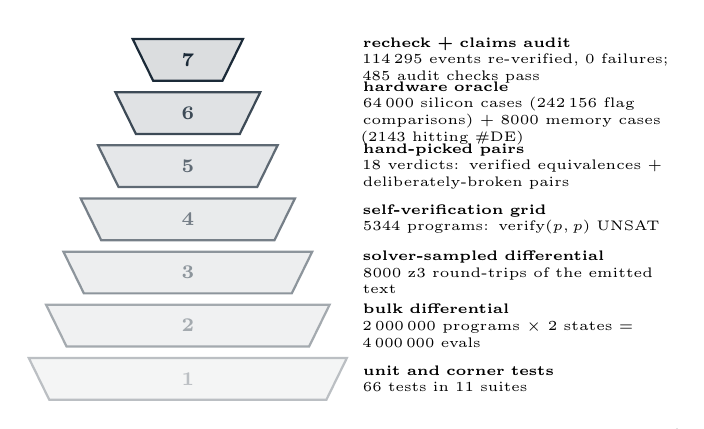
\begin{tikzpicture}[x=1cm,y=0.5cm]
  \def\pl#1#2#3#4#5{% row index (0=top), halfwidth, color, digit, annotation
    \fill[#3!16] ({-#2},{-#1*1.35}) -- ({#2},{-#1*1.35})
                 -- ({#2-0.26},{-#1*1.35-1.06}) -- ({-#2+0.26},{-#1*1.35-1.06})
                 -- cycle;
    \draw[#3, thick] ({-#2},{-#1*1.35}) -- ({#2},{-#1*1.35})
                 -- ({#2-0.26},{-#1*1.35-1.06}) -- ({-#2+0.26},{-#1*1.35-1.06})
                 -- cycle;
    \node[font=\scriptsize\bfseries, text=#3] at (0,{-#1*1.35-0.53}) {#4};
    \node[anchor=west, font=\tiny, text width=3.85cm, align=left]
        at (2.1,{-#1*1.35-0.53}) {#5};
  }
  \pl{0}{0.70}{pymcolor}{7}
     {\textbf{recheck + claims audit}\\ \RecheckTotal{} events re-verified,
      \RecheckFailed{} failures; \AuditChecks{} audit checks pass}
  \pl{1}{0.92}{pymA}{6}
     {\textbf{hardware oracle}\\ \HwCases{} silicon cases
      (\HwFlagComps{} flag comparisons) + \HwMemCases{} memory cases
      (\HwMemDef{} hitting \#DE)}
  \pl{2}{1.14}{pymB}{5}
     {\textbf{hand-picked pairs}\\ \PairVerdicts{} verdicts: verified
      equivalences + deliberately-broken pairs}
  \pl{3}{1.36}{pymC}{4}
     {\textbf{self-verification grid}\\ \GridPrograms{} programs:
      verify$(p,p)$ UNSAT}
  \pl{4}{1.58}{pymD}{3}
     {\textbf{solver-sampled differential}\\ \ZSolverQueries{} z3
      round-trips of the emitted text}
  \pl{5}{1.80}{pymE}{2}
     {\textbf{bulk differential}\\ \BulkPrograms{} programs $\times$ 2
      states = \BulkEvals{} evals}
  \pl{6}{2.02}{pymF}{1}
     {\textbf{unit and corner tests}\\ \NumTests{} tests in 11 suites}
\end{tikzpicture}
\caption{The verification pyramid, with current volumes from
\texttt{stress-compiler-full.jsonl} mode summaries, the live \texttt{recheck}
sweep, and the source tree's test count. No layer trusts another: the
concrete evaluator is checked against silicon (6), the symbolic
evaluator against the concrete (2, 3), the miter against itself (4),
hand-verified mathematics against all of the above (5), and the
reporting against the artifacts (7), with \RecheckTotal{} events
re-verified and \RecheckFailed{} failures at the start of this
document's build. Layer definitions follow the project's verification
document.}
\label{fig:pyramid}
\end{figure}

Figure~\ref{fig:pyramid} shows the seven layers and the volume at
which each currently runs. Each layer has a characteristic blind spot
that the ledger makes concrete, which is why none of them is trusted
alone.

Concrete-vs-symbolic differentials (layers 2 and 3) catch semantic
disagreement. Failures of the form ``the fold is right, the printer is
wrong'' (rows 3, 13, and 14 of the ledger) stay invisible to them,
because the constant-folded comparison never round-trips through the
emitted solver text. Layer 3 closes that gap by having z3 evaluate the
printed SMT-LIB2.

Random sampling catches large formula errors (row 11 recorded 1,733
discrepancies in one run) but has essentially zero probability at
exact boundaries. Row 15 required one hit in \ZSolverQueries{}
samples, and row 17 was caught by a hand-picked pair on its first run.

The hardware oracle checks the model against silicon, including a
\#DE pre-check protocol for division and a flag-preset protocol for
instructions that leave flags untouched. That protocol checks RFLAGS
preservation on real silicon as well as in the model.

Artifact re-derivation (layer 7) catches failures that no program
test can express. Its catches include a verifier that counted events
its own documentation described as echoed, and an audit script that
printed its verdict before checking the sections that mattered (rows
28 and 34).

\section{The Compiler Benchmark}
\label{sec:benchmark}

\subsection{Protocol}
The week-7 comparison targets the full provenance of Figure~4 of
\cite{gulwani11}: all 25 P-programs, ported to
\texttt{uint64\_t}/\texttt{int64\_t} C. Word-size scaling decisions
and two corrections of the paper's own transcription slips, each
verified against brute force, are documented in the committed sources.
Six further functions carried over from the project's sixth week. All
31 functions were compiled by \CompilerVersion{} at \mbox{-O2} and
\mbox{-O3} with \texttt{-m64} \texttt{-fno-tree-vectorize}
\texttt{-fno-tree-slp-vectorize}; the extractor for this paper asserts
that the two levels emit byte-identical assembly for every function
before the document builds. Both levels are nevertheless logged and
challenged separately: \NumBaselines{} \texttt{compiler\_baseline}
events, each carrying the compiler version, flags, C source, and
emitted assembly verbatim.

Reconciliation against the instruction subset left \NumFunctions{}
survivors. The eight exclusions (boolean tests compiled to
\texttt{setcc}-on-\texttt{\%al} plus \texttt{movzbl}, a
\texttt{testq}-based power-of-two test, the \texttt{xorl} zeroing
idiom inside an otherwise all-\texttt{cmov} three-way cycle, and
32-bit narrowing in the multiply-high decomposition) are each logged
with the actual parse error their assembly produces: sixteen
\texttt{exclusion\_confirmed} events, one per function per level. The
two opcodes the batch forced into the subset, \texttt{notq} and the
\texttt{salq} spelling of \texttt{shlq}, received the full pyramid
treatment of Section~\ref{sec:pyramid} with no exceptions.

\begin{figure*}[!t]
\centering
\begin{tikzpicture}
\begin{axis}[
  xbar, width=0.62\textwidth, height=10.6cm,
  xmin=0, xmax=21.5,
  ytick={1,...,23},
  yticklabels/.expanded=\RatioNames,
  yticklabel style={font=\scriptsize, text width=36mm, align=right},
  xlabel={gcc instruction count (identical at -O2 and -O3)},
  xlabel style={font=\small},
  legend style={at={(0.98,0.98)}, anchor=north east, legend columns=1,
                font=\scriptsize, draw=pymcolor!40, fill=white,
                fill opacity=0.9, text opacity=1, inner sep=2pt},
  every axis plot/.append style={draw=none},
  bar shift=0pt,
]
% generated by extract_data.py: literal addplot lines, no unexpanded macros
\addplot[fill=beatencolor] coordinates {(5,23) (5,22) (9,21)};
\addplot[fill=matchedcolor] coordinates {(3,20) (2,19) (2,18) (2,17) (2,16) (3,15) (3,14) (3,13) (2,12) (3,11) (2,10) (3,9) (3,8)};
\addplot[fill=honestcolor] coordinates {(5,7) (20,6) (4,5) (5,4) (4,3) (16,2) (4,1)};

\end{axis}
\end{tikzpicture}
\caption{Outcome of the compiler comparison for all \NumFunctions{}
functions, ordered beaten, matched, honest; bar length is gcc's
instruction count for that function. Generated from
\texttt{compiler-comparison-full.jsonl} (compiler\_baseline lengths; outcome
derivation identical to \texttt{audit\_claims.py}). All three wins are
verified drop-in replacements, x86-encodable and touching only
caller-clobbered registers; the seven honest no-improvements survived
MCMC budgets, and three of them additionally survived the seeded
second attempt of Section~\ref{sec:stragglers}.}
\label{fig:ratio}
\end{figure*}

\subsection{Results}
Figure~\ref{fig:ratio} shows the headline: of \NumFunctions{}
functions attempted end-to-end, gcc is beaten on \NumBeaten{}, matched
with exhaustive proofs on \NumMatched{}, and survives honestly on
\NumHonest{}. Table~\ref{tab:results} carries the per-function detail.
Every outcome class is machine-derived: the extraction script
reproduces the audit's derivation, and the ratio is a property of the
committed artifact.

\begin{table*}[!t]
\renewcommand{\arraystretch}{1.12}
\setlength{\tabcolsep}{3pt}
\caption{Per-function outcomes of the compiler comparison. ``gcc'' is
the instruction count of the emitted baseline (identical at both
levels); ``result'' is the verified shorter length where one exists.
Certificate scale is the exhaustive enumeration's rejected-candidate
count and solver queries (-O2; identical at -O3 where the universe
matches), or the search outcome for MCMC-scoped functions. Every row
derives from \texttt{compiler-comparison-full.jsonl} events
(\texttt{compiler\_baseline}, \texttt{enumeration\_summary},
\texttt{optimum}, \texttt{search\_result}); the table body is emitted
by \texttt{extract\_data.py}, not typed.}
\label{tab:results}
\centering
\scriptsize
{\rowcolors{2}{ink!2}{white}%
\renewcommand{\arraystretch}{1.12}%
\begin{tabular}{@{}l c r l r l@{}}
\toprule[0.9pt]
\rowcolor{ink!9}\sffamily\bfseries Function & \sffamily\bfseries Ref. &
\sffamily\bfseries gcc & \sffamily\bfseries outcome &
\sffamily\bfseries result & \sffamily\bfseries certificate scale / evidence \\
\midrule[0.5pt]
\ResultsTableBody
\bottomrule[0.9pt]
\end{tabular}}
\end{table*}

\subsubsection{The three wins}
Figures~\ref{fig:win-iabs} to \ref{fig:win-p19} show the verified
drop-in replacements beside gcc's own code, exactly as logged in the
artifact. Each carries a final long-timeout z3 equivalence verdict.
The iabs rewrite is the one the project reported in its sixth-week
comparison; the other two are new at scale.

\begin{figure}[!t]
\centering
\begin{minipage}[t]{0.47\columnwidth}
\centering\tiny gcc, \GccLenIabs{} instr.\par\vspace{1pt}
\lstinputlisting[style=asmstyle]{generated/gcc-iabs.asm}
\end{minipage}\hfill
\begin{minipage}[t]{0.47\columnwidth}
\centering\tiny verified, \OursLenIabs{} instr.\par\vspace{1pt}
\lstinputlisting[style=asmstyle]{generated/ours-iabs.asm}
\end{minipage}
\caption{iabs (\texttt{P9}, $|x|$): gcc computes the sign mask twice.
The verified rewrite zero-builds the accumulator, subtracts $x$
(setting flags), and selects $x$ when $-x\le 0$. Flags are read only
after \texttt{subq} writes them, which is sound under the corrected
entry-flags model (ledger row~24). From \texttt{compiler-comparison-full.jsonl}
(\texttt{compiler\_baseline}, \texttt{search\_result}), perf
\SpecPerfIabs{} to \PerfIabs{}.}
\label{fig:win-iabs}
\end{figure}

\begin{figure}[!t]
\centering
\begin{minipage}[t]{0.47\columnwidth}
\centering\tiny gcc, \GccLenPthirteen{} instr.\par\vspace{1pt}
\lstinputlisting[style=asmstyle]{generated/gcc-p13.asm}
\end{minipage}\hfill
\begin{minipage}[t]{0.47\columnwidth}
\centering\tiny verified, \OursLenPthirteen{} instr.\par\vspace{1pt}
\lstinputlisting[style=asmstyle]{generated/ours-p13.asm}
\end{minipage}
\caption{p13\_sign (\texttt{P13}, the HD sign function): doubling $x$
in \texttt{addq}~\texttt{\%rdi,\%rdi} makes CF exactly the original
sign bit, since doubling overflows if and only if the MSB was set.
\texttt{seta} yields 1 for strictly positive $x$ (CF$=0$ and ZF$=0$),
and \texttt{cmovbq} selects $-1$ when CF is set. At
$x=\mathrm{INT64\_MIN}$ the double wraps to zero (ZF set) while CF
remains set, so the two predicates still partition the sign cases
correctly. From \texttt{compiler-comparison-full.jsonl} (\texttt{search\_result},
phase optimization), perf \SpecPerfPthirteen{} to \PerfPthirteen{}.}
\label{fig:win-p13}
\end{figure}

\begin{figure}[!t]
\centering
\begin{minipage}[t]{0.47\columnwidth}
\centering\tiny gcc, \GccLenPnineteen{} instr.\par\vspace{1pt}
\lstinputlisting[style=asmstyle]{generated/gcc-p19.asm}
\end{minipage}\hfill
\begin{minipage}[t]{0.47\columnwidth}
\centering\tiny verified, \OursLenPnineteen{} instr.\par\vspace{1pt}
\lstinputlisting[style=asmstyle]{generated/ours-p19.asm}
\end{minipage}
\caption{p19\_exchange\_fields (\texttt{P19}, HD's field swap with
runtime distance $k$): gcc parks $x$ in two places, and the rewrite
holds it in \texttt{\%rax}/\texttt{\%rdi}, saving the copy. Both forms
use the variable \texttt{\%cl} shifts the subset has carried since its
first week. From \texttt{compiler-comparison-full.jsonl} (\texttt{search\_result}),
perf \SpecPerfPnineteen{} to \PerfPnineteen{}.}
\label{fig:win-p19}
\end{figure}

\subsubsection{Optimality certificates at scale}
The \NumMatched{} matched functions are proofs rather than absences of
results. The enumerator exhaustively rejected every shorter program in
each declared universe: \TotalCandidates{} candidates in total across
the \TotalOptima{} certificates of the batch (\NumMatched{} functions
at both levels, plus the week-2 suite's own \EnumCandidates{}), each
rejection backed by a logged divergence witness.
Figure~\ref{fig:candidates} shows the per-function scale of those
sweeps, spanning four orders of magnitude: \MinCandidates{}
candidates to certify \MinCandFn{} minimal, and \MaxCandidates{} for
\MaxCandFn.

\begin{figure*}[!t]
\centering
\begin{tikzpicture}
\begin{axis}[
  xbar, width=0.68\textwidth, height=8.4cm,
  xmin=100, xmax=11000000,
  xmode=log,
  log basis x=10,
  ytick={1,...,13},
  yticklabels/.expanded=\CandNames,
  yticklabel style={font=\scriptsize, text width=32mm, align=right},
  xlabel={candidates exhaustively rejected (-O2 universes; log scale)},
  xlabel style={font=\small},
  every axis plot/.append style={draw=none},
  bar shift=0pt,
]
% generated by extract_data.py: literal addplot line
\addplot[fill=matchedcolor] coordinates {(472,13) (1715,12) (1715,11) (2205,10) (2205,9) (2695,8) (139507,7) (139768,6) (139796,5) (146108,4) (555680,3) (871298,2) (5104879,1)};

\end{axis}
\end{tikzpicture}
\caption{The scale of the optimality certificates for the
\NumMatched{} matched functions: the number of candidate programs the
enumerator evaluated and rejected, each with a logged witness, before
concluding that no shorter equivalent exists in the declared universe.
Generated from \texttt{enumeration\_summary.candidates\_total} events
in \texttt{compiler-comparison-full.jsonl} (-O2).}
\label{fig:candidates}
\end{figure*}

\subsection{The stragglers' second attempt}
\label{sec:stragglers}
Three functions had survived their search budgets in the project's
sixth week without improvement. The protocol requires a serious second
attempt rather than a silent repeat, so each received seeded
synthesis: \StragglerChains{} chains of \StragglerSeconds{}~s per
level, against a primary pass whose logged chain wall-clock medians
are \MedianOptChainSec{}~s (optimization) and \MedianSynthChainSec{}~s
(synthesis). The second attempt is therefore 2.5 times the primary
optimization and five times the primary synthesis budget per chain.
Chains start from structural variations of the compiler's own form
(the identity, single-instruction deletions, and adjacent swaps)
rather than from random programs. The rationale and per-chain starts
are logged in \texttt{straggler\_plan} and \texttt{seeded\_start}
events. Table~\ref{tab:stragglers} records the outcome from the logged
summaries: no verified improvement from informed starts either. gcc's
forms for these three survive the second attempt at both levels, and
that is reported as the result.

\begin{table}[!t]
\renewcommand{\arraystretch}{1.15}
\setlength{\tabcolsep}{4pt}
\caption{The stragglers' second attempt (seeded synthesis,
\StragglerChains{} chains $\times$ \StragglerSeconds{}~s per level).
From \texttt{straggler\_summary} events in \texttt{compiler-comparison-full.jsonl}.}
\label{tab:stragglers}
\centering
\scriptsize
{\rowcolors{2}{ink!2}{white}%
\renewcommand{\arraystretch}{1.18}%
\begin{tabular}{@{}l r r l@{}}
\toprule[0.9pt]
\rowcolor{ink!9}\sffamily\bfseries benchmark & \sffamily\bfseries spec perf &
\sffamily\bfseries best found & \sffamily\bfseries status \\
\midrule[0.5pt]
\StragglerTableBody
\bottomrule[0.9pt]
\end{tabular}}
\end{table}

\subsection{Calibration: making the comparison mean something}
\label{sec:calibration}
Two of the three wins above were not the first wins found. The
difference between them records what the calibration pass changed. The first
full-scale run claimed the popcount program with a 14-instruction
rewrite, and the second run claimed the sign function with a
4-instruction one. Reading those claimed winners against the real
machine, before reporting either, showed that both licensed forms the
hardware does not have.

The popcount winner used \texttt{andq} with 64-bit immediates in three
of its forms. Real ALU instructions take only sign-extended 32-bit
immediates, which is why gcc had materialized those constants with
\texttt{movabsq}. As actual instructions the winner was 17 programs
long, worse than gcc. The search had instruction forms that the
compiler's output structurally cannot contain, so the comparison was
weighted in our favor.

The sign-function winner held its $-1$ in \texttt{\%rsp}. In the
model, where all sixteen registers are equal and the live-out is RAX,
this is equivalent, and the solver proved it. A real function body
that sets RSP returns through the wrong address. Equivalent programs
and equivalent functions diverge exactly when a candidate writes a
callee-saved or stack register.

Both were fixed to make the two notions of equivalence coincide by
construction. The searched subset now admits only imm32-encodable ALU
immediates (full-width constants must be materialized via
\texttt{movq}, as gcc does) and only caller-clobbered register
destinations. The model itself stays permissive, because committed
rejection witnesses from earlier universes replay through it and must
keep re-checking. The comparison was then re-adjudicated from scratch.
The popcount win vanished (the function is now an honest
no-improvement), while the sign-function win was found again, cleanly,
as a different 4-instruction construction using a scratch register
(Fig.~\ref{fig:win-p13}). The claims audit enforces both contracts on
every claimed program, so the calibration is checked rather than
remembered. The week-2 certificate suite was regenerated through each
universe change: \EnumChainA{} candidates, then \EnumChainB{}, then
\EnumChainC{}, then \EnumChainD{}, with byte-identical optima each
time.

\section{Lessons Learned}
\label{sec:lessons}

\begin{table*}[!t]
\renewcommand{\arraystretch}{1.18}
\setlength{\tabcolsep}{4pt}
\caption{A selection of the \NumLedgerRows{}-row defect ledger. The
thirteen rows shown are selected for instructiveness, and the text is
abridged to first sentences; the full ledger is a committed project
document. Every row is machine-extracted from that document by
\texttt{extract\_data.py}, so the selection, not the content, is
editorial.}
\label{tab:ledger}
\centering
\scriptsize
{\rowcolors{2}{ink!2}{white}%
\renewcommand{\arraystretch}{1.16}%
\begin{tabular}{@{}r p{0.30\textwidth} p{0.15\textwidth} p{0.29\textwidth}@{}}
\toprule[0.9pt]
\rowcolor{ink!9}\sffamily\bfseries \# & \sffamily\bfseries bug &
\sffamily\bfseries caught by & \sffamily\bfseries why the other layers missed it \\
\midrule[0.5pt]
\LedgerTableBody
\bottomrule[0.9pt]
\end{tabular}}
\end{table*}

The ledger (Table~\ref{tab:ledger}) records the project's defects and
the layer that caught each one. Its rows cluster into failure shapes.

\subsubsection{The story is not the artifact}
Rows 22 and 23 are the founding incidents: a correct machine result
mis-transcribed into a report, and a discovery whose evidence was
destroyed by the debugging workflow around it. External verification
of claims the pipeline had already blessed found both. They produced
the artifact-of-record rule that everything else here descends from.

\subsubsection{The fold is right, the printer is wrong}
Rows 3, 13, and 14 share a shape: the constant-folded semantics agreed
with concrete evaluation everywhere, while the emitted solver text was
wrong. Concrete-vs-symbolic testing cannot see this, because it never
round-trips through the printed text. This is why layer 3 of the
pyramid exists.

\subsubsection{A sound model is not a well-tested model}
Rows 24, 32, and 33 are the calibration incidents of
Section~\ref{sec:calibration}, together with the entry-flags
correction that compiler integration forced in week 6. Each is a model
in which every test passes because the tests share the model's blind
spot. Each was found only by confronting the model with something
outside it: real compiler output, the ISA's encoding rules, or the
calling convention.

\subsubsection{Tests that cannot fail}
Row 29 records a documented opcode acceptance whose pinning test
contained a fallback that made it pass exactly when the claim was
false. The ADR said it worked, the test said it worked, and the parser
rejected every real instance. The un-neutered form of the test found
the bug the same day the batch first emitted the opcode.

\subsubsection{The verifier needs verifying}
Rows 28 and 34 live in the observability layer: an event counter whose
totals did not decompose to what it validated, and an audit script
that printed its verdict before running the sections that mattered.
The ledger's throughline, stated at the project's week-6 close and
kept verbatim since: \emph{a sound model and a well-tested model are
different things, and ``every test passes'' is a claim about the
model, not the world.}

The distribution of catchers argues for the pyramid's shape. Unit
tests caught corner arithmetic that the random layers rarely reach.
The bulk differential caught the release-mode panic that weeks of
corner tests had missed (row 27). Solver sampling caught printer bugs.
A hand-picked pair caught a one-in-$2^{64}$ boundary that
\ZSolverQueries{} random samples had never touched. Silicon caught no
semantics bugs, because the model was right, but its \#DE protocol
caught oracle bugs instead (row 7). The artifact layer caught the
reporting failures that no program-level test can even express.

\section{Limitations}
\label{sec:limitations}

The claims of this paper are scoped, and the scopes are load-bearing.

\begin{itemize}
\item \textbf{Optimality is relative to a declared universe.} The
enumerator proves that no shorter equivalent exists among the declared
registers, immediates, and forms; the universe is logged with every
certificate. No global claims are made, and the \NumMatched{} matches
are matches within those universes.
\item \textbf{Straight-line code only.} Branches and loops are excluded
at the parse layer, where a local label is a hard error. The project's
own week-6 hand-written cycle function was excluded for this boundary.
No week-7 exclusion was control-flow, but that is fortune rather than
reach: gcc happened to compile the entire batch branchlessly, and any
function it compiles with a branch falls outside the model.
\item \textbf{64-bit registers only.} The partial-register ban, the
project's oldest rule, excluded seven of the eight week-7
non-survivors (booleans compiled through \texttt{setcc} on
\texttt{\%al} and \texttt{movzbl}, and the
\texttt{xorl}/\texttt{andl}/\texttt{movl} narrowing idioms). The
eighth, the power-of-two test, fell to \texttt{testq}, a flags-only
opcode outside the subset. All eight exclusions are empirically
confirmed against the committed assembly.
\item \textbf{Equivalence is a solver claim.} z3's UNSAT verdicts are
labeled as solver claims throughout. \texttt{recheck} validates
everything around them (testcases, witnesses, cost-zero on committed
sets) and never pretends to concretely re-check an equivalence.
\item \textbf{Latency is a static table.} The perf metric is a
per-opcode latency table rather than measured cycles; the instruction
count comparisons shown for the wins are count-level claims.
\item \textbf{One compiler, one machine.} \CompilerVersion{} is the
only compiler compared, and the comparison would need re-running per
compiler release. Both optimization levels were compared despite
emitting identical code, which is logged rather than assumed.
\end{itemize}

\section{Future Work}
\label{sec:future}

Two exclusions dominate the loss rate at scale, and they are the next
frontiers.

\subsubsection{Partial-register support} The 32-bit and 8-bit
sub-register semantics that the v0 ban rejects are well-defined on
real hardware. Modeling them soundly (zero-extension on write, the
\texttt{\%al}-within-\texttt{\%rax} aliasing, and the x86-64
partial-register stalls) would return eight benchmark functions to the
comparison, including the three-value cycle whose emitted code is
otherwise entirely \texttt{cmov}s. The cost is real: every new opcode
form in this project earned a full pyramid treatment before it could
appear in any claim, and sub-register semantics multiply the aliasing
surface of every existing test.

\subsubsection{Control flow} The straight-line model excludes branches
by design. The \texttt{je}-shaped exclusions, and every real-world
function with a loop, need a bounded-control-flow model: basic blocks
with structured merge points, or the loop-free-program formulation of
\cite{gulwani11} itself, before the comparison can leave the Hacker's
Delight genre. The certificate infrastructure (witnesses, replay,
recheck) transfers unchanged; the miter does not.

Beyond these, three directions follow from the current design. Learned
latency from hardware counters would replace the static table, as
STOKE's original methodology did \cite{stoke13}. Testcase broadcasting
across parallel chains would improve search efficiency. Extending the
compiled-binary oracle to the new frontiers would repeat, for control
flow and partial registers, what the project's fourth week did for
division and memory.

\section{Conclusion}
\label{sec:conclusion}

This paper reports a superoptimizer that beats a production compiler
on \NumBeaten{} of \NumFunctions{} real benchmark functions with
verified, encodable, ABI-clean drop-in replacements, proves
\NumMatched{} more optimal within declared universes totaling
\TotalCandidates{} rejected candidates, and reports honestly on the
rest, three of them after a five-times-budget informed-start second
attempt. The center of the work is the discipline that makes those
numbers meaningful: a seven-layer pyramid in which every layer assumes
the others are wrong, an artifact pipeline that re-derives every claim
from committed logs (and re-verified \RecheckTotal{} events with zero
failures as the first step of building this document), and a
\NumLedgerRows{}-row ledger that records, in the project's own voice,
every way the story diverged from the artifact until the pipeline made
the divergence impossible to hide.

The benchmark result and the ledger describe one finding. Search finds
what compilers miss, and reporting discipline is what makes the
finding real. Inspecting the artifact is what separates a result from
a claim.

\begin{thebibliography}{99}
% IEEEtran's thebibliography already calls \sloppy (hfuzz=0.5pt);
% widen the declared tolerance to 1pt so a sub-point line cannot trip
% the overfull warning. No visual effect at 0.19mm.
\hfuzz=1pt

\bibitem{massalin87}
H.~Massalin, ``Superoptimizer: A look at the smallest program,''
in \emph{Proc.\ Second Int'l Conf.\ on Architectural Support for
Programming Languages and Operating Systems (ASPLOS~II)}, 1987,
pp.~122--127.

\bibitem{denali02}
R.~Joshi, G.~Nelson, and K.~Randall, ``Denali: A goal-directed
superoptimizer,'' in \emph{Proc.\ Int'l Conf.\ on Architectural
Support for Programming Languages and Operating Systems (ASPLOS~X)},
2002, pp.~304--314.

\bibitem{gulwani11}
S.~Gulwani, S.~Jha, A.~Tiwari, and R.~Venkatesan, ``Synthesis of
loop-free programs,'' in \emph{Proc.\ 32nd ACM SIGPLAN Conf.\ on
Programming Language Design and Implementation (PLDI)}, 2011,
pp.~62--73.

\bibitem{stoke13}
E.~Schkufza, R.~Sharma, and A.~Aiken, ``Stochastic superoptimization
of x86 binaries,'' in \emph{Proc.\ 18th Int'l Conf.\ on Architectural
Support for Programming Languages and Operating Systems (ASPLOS~XVIII)},
2013, pp.~305--316.

\bibitem{warren13}
H.~S.~Warren, \emph{Hacker's Delight}, 2nd~ed. Addison-Wesley, 2013.

\bibitem{z3}
L.~de~Moura and N.~Bj{\o}rner, ``Z3: An efficient SMT solver,'' in
\emph{Proc.\ Tools and Algorithms for the Construction and Analysis of
Systems (TACAS)}, 2008, pp.~337--340.

\bibitem{sysvabi}
System~V Application Binary Interface, AMD64 Architecture Processor
Supplement, Draft~1.0, AMD64 Systems Community, 2023.

\bibitem{intel-sdm}
Intel~64 and IA-32 Architectures Software Developer's Manual,
Combined Volumes 1--4, Intel Corp., 2024.

\bibitem{bansal06}
S.~Bansal and A.~Aiken, ``Automatic generation of peephole
superoptimizers,'' in \emph{Proc.\ 12th Int'l Conf.\ on Architectural
Support for Programming Languages and Operating Systems (ASPLOS~XII)},
2006.

\bibitem{bansal08}
S.~Bansal and A.~Aiken, ``Binary translation using peephole
superoptimizers,'' in \emph{Proc.\ 8th USENIX Symp.\ on Operating
Systems Design and Implementation (OSDI)}, 2008, pp.~177--192.

\bibitem{souper}
R.~Sasnauskas, Y.~Chen, P.~Collingbourne, J.~Ketema, G.~Lup,
J.~Taneja, and J.~Regehr, ``Souper: A synthesizing superoptimizer,''
arXiv:1711.04422, 2017.

\bibitem{pnueli98}
A.~Pnueli, M.~Siegel, and E.~Singerman, ``Translation validation,'' in
\emph{Proc.\ Tools and Algorithms for the Construction and Analysis of
Systems (TACAS)}, LNCS~1384, 1998, pp.~151--166.

\bibitem{emi14}
V.~Le, M.~Afshari, and Z.~Su, ``Compiler validation via equivalence
modulo inputs,'' in \emph{Proc.\ 35th ACM SIGPLAN Conf.\ on Programming
Language Design and Implementation (PLDI)}, 2014.

\bibitem{alive2}
N.~P.~Lopes, J.~Lee, C.-K.~Hur, Z.~Liu, and J.~Regehr, ``Alive2:
Bounded translation validation for LLVM,'' in \emph{Proc.\ 42nd ACM
SIGPLAN Int'l Conf.\ on Programming Language Design and Implementation
(PLDI)}, 2021.

\bibitem{x86sem}
S.~Dasgupta, D.~Park, T.~Kasampalis, V.~S.~Adve, and G.~Ro\c{s}u,
``A complete formal semantics of x86-64 user-level instruction set
architecture,'' in \emph{Proc.\ 40th ACM SIGPLAN Conf.\ on Programming
Language Design and Implementation (PLDI)}, 2019.

\bibitem{stokefp14}
E.~Schkufza, R.~Sharma, and A.~Aiken, ``Stochastic optimization of
floating-point programs with tunable precision,'' in \emph{Proc.\ 35th
ACM SIGPLAN Conf.\ on Programming Language Design and Implementation
(PLDI)}, 2014.

\bibitem{chlorophyll14}
P.~M.~Phothilimthana \emph{et al.}, ``Chlorophyll: Synthesis-aided
compiler for low-power spatial architectures,'' in \emph{Proc.\ 35th
ACM SIGPLAN Conf.\ on Programming Language Design and Implementation
(PLDI)}, 2014, pp.~396--407.

\bibitem{sygus13}
R.~Alur, R.~Bod{\'\i}k, G.~Juniwal, M.~M.~K.~Martin, M.~Raghothaman,
S.~A.~Seshia, R.~Singh, A.~Solar-Lezama, E.~Torlak, and A.~Udupa,
``Syntax-guided synthesis,'' in \emph{Proc.\ Formal Methods in
Computer-Aided Design (FMCAD)}, 2013.

\bibitem{sketch06}
A.~Solar-Lezama, L.~Tancau, R.~Bodik, S.~Seshia, and V.~Saraswat,
``Combinatorial sketching for finite programs,'' in \emph{Proc.\ 12th
Int'l Conf.\ on Architectural Support for Programming Languages and
Operating Systems (ASPLOS~XII)}, 2006.

\bibitem{rosette14}
E.~Torlak and R.~Bodik, ``A lightweight symbolic virtual machine for
solver-aided host languages,'' in \emph{Proc.\ 35th ACM SIGPLAN Conf.\
on Programming Language Design and Implementation (PLDI)}, 2014.

\bibitem{flashmeta15}
O.~Polozov and S.~Gulwani, ``FlashMeta: A framework for inductive
program synthesis,'' in \emph{Proc.\ ACM SIGPLAN Int'l Conf.\ on
Object-Oriented Programming, Systems, Languages, and Applications
(OOPSLA)}, 2015.

\bibitem{gulwani-survey17}
S.~Gulwani, O.~Polozov, and R.~Singh, ``Program synthesis,''
\emph{Foundations and Trends in Programming Languages}, vol.~4,
no.~1--2, pp.~1--119, 2017.

\bibitem{cvc4}
C.~Barrett, C.~L.~Conway, M.~Deters, L.~Hadarean, D.~Jovanovi{\'c},
T.~King, A.~Reynolds, and C.~Tinelli, ``CVC4,'' in \emph{Proc.\ 23rd
Int'l Conf.\ on Computer Aided Verification (CAV)}, 2011.

\bibitem{cvc5}
H.~Barbosa \emph{et al.}, ``cvc5: A versatile and industrial-strength
SMT solver,'' in \emph{Proc.\ 28th Int'l Conf.\ on Tools and Algorithms
for the Construction and Analysis of Systems (TACAS)}, 2022.

\bibitem{beaver09}
S.~K.~Jha, S.~A.~Seshia, and R.~Somenzi, ``Beaver: Engineering an
efficient SMT solver for bit-vector arithmetic,'' in \emph{Proc.\ 21st
Int'l Conf.\ on Computer Aided Verification (CAV)}, LNCS~5643, 2009,
pp.~668--674.

\bibitem{arrays01}
A.~Stump, C.~W.~Barrett, D.~L.~Dill, and J.~Levitt, ``A decision
procedure for an extensional theory of arrays,'' in \emph{Proc.\ 16th
Annual IEEE Symp.\ on Logic in Computer Science (LICS)}, 2001.

\bibitem{dutertre06}
B.~Dutertre and L.~de~Moura, ``A fast linear-arithmetic solver for
DPLL(T),'' in \emph{Proc.\ 18th Int'l Conf.\ on Computer Aided
Verification (CAV)}, LNCS~4144, 2006.

\bibitem{nieuwenhuis06}
R.~Nieuwenhuis, A.~Oliveras, and C.~Tinelli, ``Solving SAT and SAT
modulo theories: From an abstract Davis--Putnam--Logemann--Loveland
procedure to DPLL(T),'' \emph{J.\ ACM}, vol.~53, no.~6,
pp.~937--977, 2006.

\bibitem{mathsat05}
M.~Bozzano, R.~Bruttomesso, A.~Cimatti, T.~Junttila, P.~van~Rossum,
S.~Schulz, and R.~Sebastiani, ``MathSAT: Tight integration of SAT and
mathematical decision procedures,'' \emph{J.\ Automated Reasoning},
vol.~35, pp.~265--293, 2005.

\bibitem{smt-handbook18}
C.~Barrett, R.~Sebastiani, S.~A.~Seshia, and C.~Tinelli,
``Satisfiability modulo theories,'' in \emph{Handbook of
Satisfiability}, 2nd~ed. IOS Press, 2021, ch.~33, pp.~1267--1329.

\bibitem{kroening08}
D.~Kroening and O.~Strichman, \emph{Decision Procedures: An
Algorithmic Point of View}. Springer, 2008.

\bibitem{nec00}
G.~C.~Necula, ``Translation validation for an optimizing compiler,''
in \emph{Proc.\ ACM SIGPLAN Conf.\ on Programming Language Design and
Implementation (PLDI)}, 2000.

\bibitem{leroy09}
X.~Leroy, ``Formal verification of a realistic compiler,''
\emph{Commun.\ ACM}, vol.~52, no.~7, pp.~107--115, 2009.

\bibitem{csmith11}
X.~Yang, Y.~Chen, E.~Eide, and J.~Regehr, ``Finding and understanding
bugs in C compilers,'' in \emph{Proc.\ 32nd ACM SIGPLAN Conf.\ on
Programming Language Design and Implementation (PLDI)}, 2011.

\bibitem{vellvm12}
J.~Zhao, S.~Nagarakatte, M.~M.~K.~Martin, and S.~Zdancewic,
``Formalizing the LLVM intermediate representation for verified
program transformations,'' in \emph{Proc.\ 39th ACM
SIGPLAN-SIGACT Symp.\ on Principles of Programming Languages (POPL)},
2012, pp.~427--440.

\bibitem{x86isa17}
S.~Goel, W.~A.~Hunt, Jr., and M.~Kaufmann, ``Engineering a formal,
executable x86 ISA simulator for software verification,'' in
\emph{Provably Correct Systems}. Springer, 2017, pp.~173--209.

\bibitem{x86tso10}
P.~Sewell, S.~Sarkar, S.~Owens, F.~Z.~Nardelli, and M.~O.~Myreen,
``x86-TSO: A rigorous and usable programmer's model for x86
multiprocessors,'' \emph{Commun.\ ACM}, vol.~53, no.~7, pp.~89--97,
2010.

\bibitem{mckeeman98}
W.~M.~McKeeman, ``Differential testing for software,''
\emph{Digital Technical Journal}, vol.~10, no.~1, pp.~100--107, 1998.

\bibitem{groce07}
A.~Groce, G.~Holzmann, and R.~Joshi, ``Randomized differential
testing as a prelude to formal verification,'' in \emph{Proc.\ 29th
Int'l Conf.\ on Software Engineering (ICSE)}, 2007.

\bibitem{regehr12}
J.~Regehr, Y.~Chen, P.~Cuoq, E.~Eide, C.~Ellison, and X.~Yang,
``Test-case reduction for C compiler bugs,'' in \emph{Proc.\ 33rd ACM
SIGPLAN Conf.\ on Programming Language Design and Implementation
(PLDI)}, 2012.

\bibitem{chen13}
Y.~Chen, A.~Groce, C.~Zhang, W.-K.~Wong, X.~Fern, E.~Eide, and
J.~Regehr, ``Taming compiler fuzzers,'' in \emph{Proc.\ 34th ACM
SIGPLAN Conf.\ on Programming Language Design and Implementation
(PLDI)}, 2013.

\bibitem{quickcheck00}
K.~Claessen and J.~Hughes, ``QuickCheck: A lightweight tool for
random testing of Haskell programs,'' in \emph{Proc.\ Fifth ACM
SIGPLAN Int'l Conf.\ on Functional Programming (ICFP)}, 2000.

\bibitem{smtlib10}
C.~Barrett, A.~Stump, and C.~Tinelli, ``The SMT-LIB standard:
Version 2.0,'' Dept.\ of Computer Science, The University of Iowa,
Tech.\ Rep., 2010.

\bibitem{amd-apm}
Advanced Micro Devices, \emph{AMD64 Architecture Programmer's
Manual, Volume 1: Application Programming}, AMD Publication 24592.

\bibitem{fog-tables}
A.~Fog, ``Instruction tables: Lists of instruction latencies,
throughputs and micro-operation breakdowns for Intel, AMD and VIA
CPUs,'' Technical University of Denmark, 2024.

\end{thebibliography}

\end{document}
